% Fig. 1 (converted from epsf/figure1; graphic from plots/wi.eps -> images/wi.pdf)
\topinsert
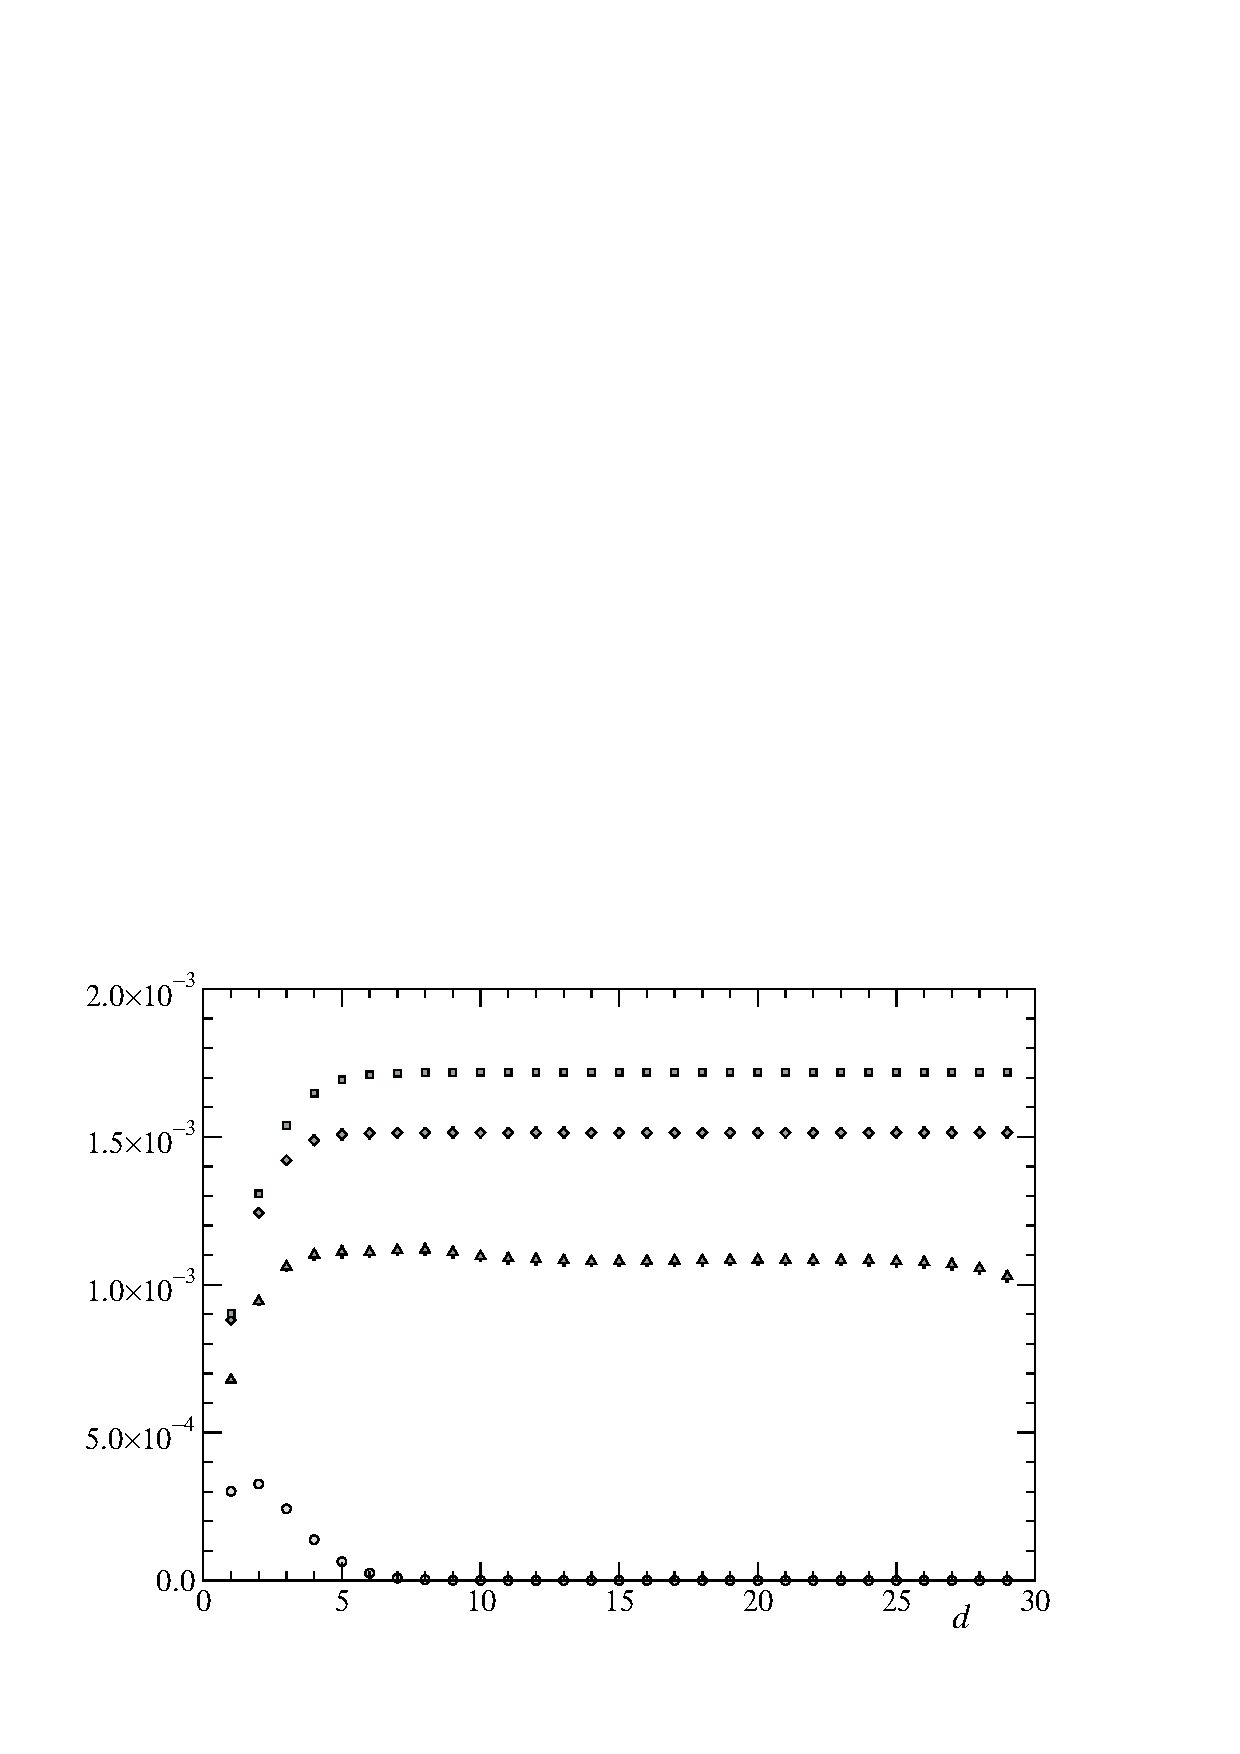
\includegraphics[width=10.5cm]{images/wi}
\vspace{0.3cm}
\figurecaption{%
Combinations of correlation functions appearing
in the PCAC relation (8.8),
plotted as a function of the summation range $d$.
The linear combinations of correlation functions shown
are the ones multiplying the renormalization constant $\ZAh{ud}$ (triangles),
the improvement coefficient $\cfl$ (diamonds)
and the factor $1-\ZAh{ud}\ctp m_{ud}$ (squares)
at flow time $t=3.86$.
For $d\geq9$, the function
$\CAtP{ud}$ (circles) is many orders of magnitude smaller than the other
functions and can be safely neglected (cf.~subsect.~8.1).
All quantities are given in lattice units.
}
\endinsert
